%%%%%%%%%%%%%%%%%%%%%%%%%%%%%%%%%%%%%%%%%%%%%%%%%%%%%%%%%%%%%%%%%%%%%%%%%%%%%%%%
%% SECTION
%%%%%%%%%%%%%%%%%%%%%%%%%%%%%%%%%%%%%%%%%%%%%%%%%%%%%%%%%%%%%%%%%%%%%%%%%%%%%%%%
\section{\textcolor{green}{Historia do samba}}\index{Historia do samba}
O samba como principal manifestação da cultura brasileira está bem reconhecida no Brasil do seculo XXI;
porem, o caminho da palavra samba, ou da ideia do samba, inicia muito tempo atrás;
pois como mostraremos mais adiante, existiu uma transição entre os termos ``batuque'' e ``samba''.
Nos inícios do seculo XIX
se designava com a palavra ``batuque''  a qualquer reunião de ``pretos'' (em expressões próprias da época) realizando danças entendidas como africanas\footnote{
Porem no Brasil existem registros desta palavra desde o século XVIII \cite[pp. 85]{sandroni2001feitico}. }
\cite[pp. 54]{de4danccas} \cite[pp. 73]{lara2007memoria}.
Um exemplo disto pode ser visto numa carta ao redator do ``Correio Braziliense''  (Londres, ING),
sobre os negócios públicos em Pernambuco,
escrita o dia 3 de dezembro do 1816, e publicada em 1817 \cite[pp. 468]{batuqueBraziliense},
onde se menciona\footnote{\label{footort}A forma da escrita corresponde ao texto original}:
\begin{citando}%%
Quasi dous annos depois, o Ouvidor das Alagoas, que não tinha tido parte neste Drama,
sonhou com outro levante de pretos na sua comarca, 
fundamentado unicamente em um \textbf{batuque} de dança, 
que alguns faziam nas inmmediaçoens de um Engenho de assucar, ...
\end{citando} 
Pelo que se observa, 
a palavra ``batuque'' não se usava para referenciar a uma dança em particular e sim aos festejos dos negros em geral \cite[pp. 85]{sandroni2001feitico}.

\PRLsep{*}

Paralelamente na historia, a palavra samba estava iniciando a ser usada como parte
das expressões nestos festejos populares. 
Isto pode ser visto na ordem do dia do Quartel do Governo das Armas em
Pernambuco, 8 de julho de 1830, publicado no jornal ``Diario de Pernambuco''(PE), 
onde se  relata\footref{footort} \cite[pp. 3]{sambadiariodepernanbuco}:
\begin{citando}%%
Naõ existindo fora da Capital nos diferentes pontos,
onde se achão destacadas as Companhias deste Corpo, 
hum serviço ativo, a que sejão ellas forçadas, 
necessariamente a occiozidade dispora' 
aos mais bem conduzidos a se entreterem nas pescarias de curraes e trapaçoens de coqueiros,
em cujos passatempos sera' recebida com agrado a viola, e o \textbf{samba};
e aos peraltas, cada vez os fara' mais dezenvolvidos na conjugação do verbo surripio.
\end{citando}
Anos posteriores podemos encontrar uma dualidade no uso da palavra samba, 
tanto no sentido de música como de dança; por exemplo, no jornal ``O Capuceiro''(PE),
do dia 3 de fevereiro de 1838, temos uma referencia ao samba como música,
onde ademais se ressalta a beleza da interpretação musical;
o seguinte é um fragmento desse texto\footnote{\label{footort2}A forma da escrita corresponde ao texto original} \cite[pp. 1]{sambaperiodicoocapuceiro}:
\begin{citando}%%
Segue se, que tão perfeita na Cantoria era Catalini, ou a Pasta,
como pai Antonio descantando no seu birimbau; que tanto val huma garatuja da China,
que vinhão nos bules, e bandejas,
como as pinturas de Rafael, de Rubens, ou do Corregio;
que tão agradavel he hum \textbf{samba} d'almocreves, como a Semiramis,
a Gaza-ladra, o Tencredi, \&c. de Rossini, ...
\end{citando}
Também podemos achar outra referencia do samba no sentido musical, no jornal ``Diário do Rio de Janeiro''(RJ),
do dia 19 de abril de 1939, onde se menciona\footref{footort2} \cite[pp. 1]{sambadiariorj1}:
\begin{citando}%%
Em quanto o cortezão, o palaciano, o gamenho, o literato, o magistrado etc., 
espancão melanconias, desvanecem cuidados tomando em ricas bocetas o cheiroso rapé;
o laborioso maluto, a quem furtárão o cavalinho (que é a menina dos seos olhos)
depois de affligir-se, e praguejar em balde arranca do quijeje (bolso na celoura)
o encebado cornimboque, saca lhe com estalo e tapadoura, e chafurdando as ventas em duas,
ou trez pitadas mestras da sua torradinha, esquece-se do cavallo, resigna-se com sua sorte,
e com uma viola nas unhas zangarrêa o \textbf{samba} por uma noite inteira.
\end{citando}
Por outro lado, temos uma referencia ao samba relacionando-o com a dança, no jornal ``O Capuceiro''(PE),
do dia 12 de novembro de 1842\footnote{Só 6 anos apos referenciar o samba como música, 
no mesmo jornal, é usado o mesmo termo agora relacionado com a dança.}, 
onde mencionam\footref{footort2} \cite[pp. 5]{sambaperiodicoocapuceiro2}:
\begin{citando}%%
Aqui pelo nosso mato,\\
Qn'stava então mui tatamba,\\
Não se sabia outra cousa,\\
Senão a \textbf{dansa do samba}.
\end{citando}
Neste ultimo texto vemos que ainda se diz a \textbf{dança do samba} e não dançar o samba,
mas é possível observar como o termo vai se fusionando com a dança.
Seguindo esta linha de pensamento, 
podemos ver outro exemplo no Jornal ``O Guaycuru''(BA), do dia 26 de maio de 1846,
onde podemos ler o seguinte texto\footref{footort2} \cite[pp. 2]{sambaperiodicooguaycuru}:
\begin{citando}%%
Todavia o famigerado Salles, sem respeito algum aos institutos de sua ordem, 
foi-se pòr na Cachoeira a divertir talvez \textbf{dançando o samba}...
Que bello exemplar da vida religiosa!?
\end{citando}
Como tem sido visto, 
para esta data já se podia ver como as pessoas entendiam o samba como uma dança.
Porem, não terá que se esperar muito pra achar referencias mostrando ao samba
como uma expressão cultural em si mesma, 
uma declaração deste tipo pode ser achada no jornal ``O Cosmorama na Bahia'' (BA), 
no dia 15 de dezembro de 1849, onde menciona\footref{footort2} \cite[pp. 2]{sambaperiodicoocosmorama}:
\begin{citando}%%
Cousa já muito antiga para engordar os patinhos. 
Para o espectaculo seguinte haverá um \textbf{SAMBA} á moda da Bahia, 
em que entram os negreiros todos.
\end{citando}

\PRLsep{*}
Retomando o tema do batuque

\PRLsep{*}


Assim, como mostrado anteriormente e resumindo as ideias, 
na literatura do Brasil já temos referencias da palavra ``samba'' desde o ano de 1830; 
porem como menciona Sandroni C. no seu livro ``Feitiço decente: transformações do samba no Rio de Janeiro'', 
falando especificamente do Rio de Janeiro, 
a palavra samba foi pouco conhecida ate o último quartel do século XIX \cite[pp. 86]{sandroni2001feitico};
este dado cobrará importância quando o termo seja relacionado com as gafieiras.
Por outro lado, a palavra  ``batuque'' usada para designar festejos populares com danças, foi muito recorrente ate inícios do seculo XX, 
onde a palavra ``samba'' virou mais popular para descrever estas atividades \cite[pp. 85]{sandroni2001feitico} \cite[pp. 47]{diniz2008almanaque}; 
a Figura \ref{fig:sambacrono} descreve o uso destas palavras ao longo do tempo.
\begin{figure}[h]
  \centering
    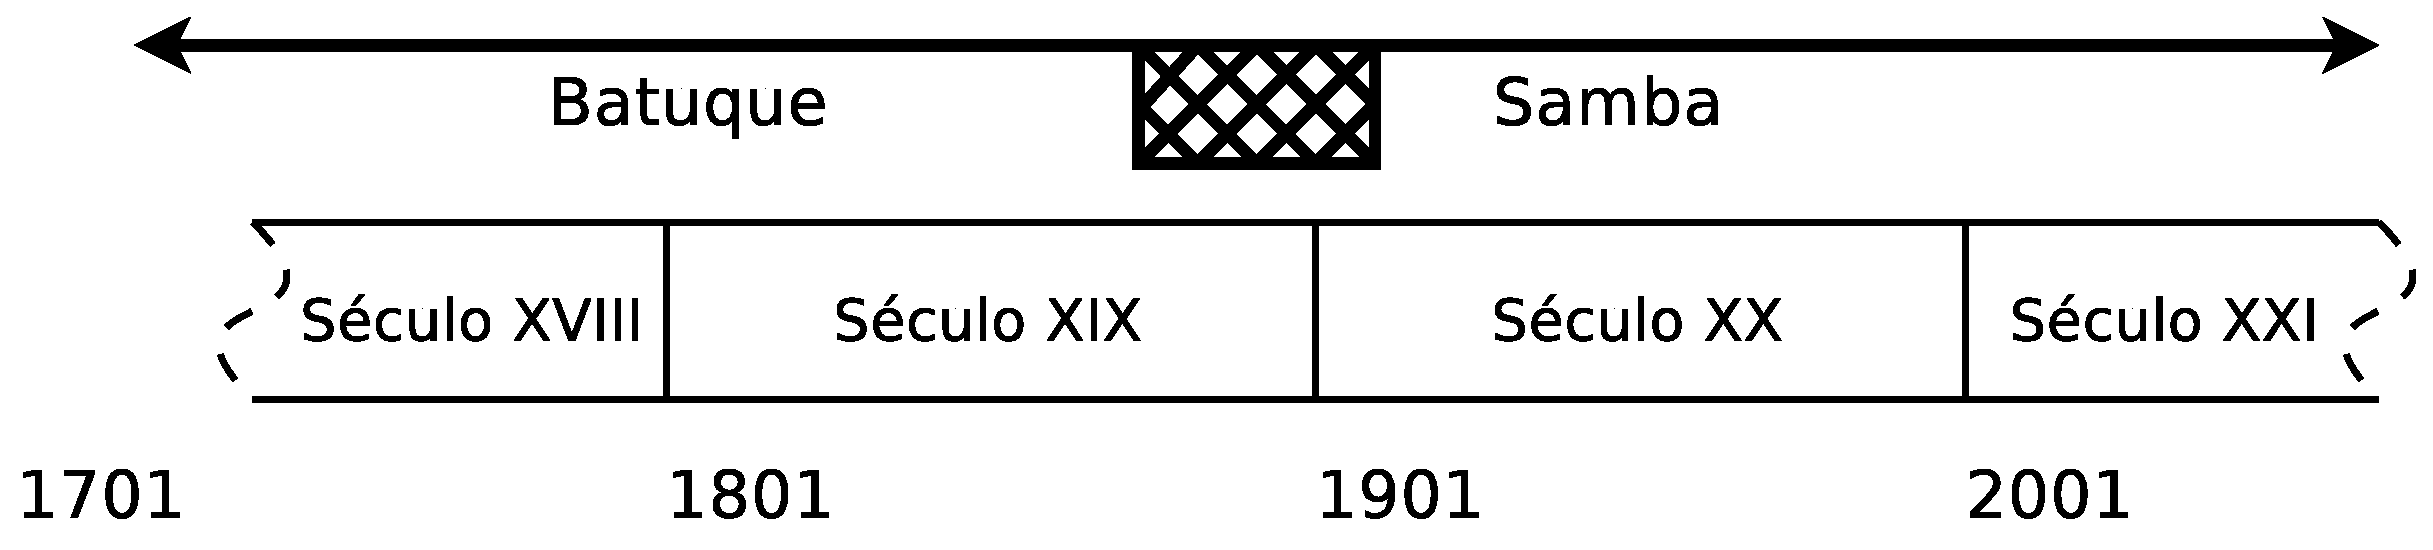
\includegraphics[width=0.85\textwidth]{chapters/cap-historia/samba-crono.eps}
  \caption{Cronologia da designação geral dos festejos de pessoas, de raça negra, no Brasil.}
  \label{fig:sambacrono}
\end{figure}


Entre as explicações da origem da palavra ``samba'', 
a mais conhecida, é a que promove que esta vem do idioma quimbundo, 
sendo derivado da palavra ``semba''  que significa umbigada \cite[pp. 47]{diniz2008almanaque} \cite[pp. 50]{da2015historia}.
Uma referencia muito conhecida deste vinculo é a descrita no livro ``O negro e o garimpo em Minas Gerais''
de Mata Machado Filho, onde ele comenta que ``os negros corrigem para semba se 
alguém lhes fala em samba'' \cite[pp. 85]{sandroni2001feitico}. Assim se vê que existe
desde antanho uma relação entre as palavras, 
samba, semba e umbigada.

\begin{comment}
Entre as danças "profanas" \cite[pp. 85]{sandroni2001feitico} afro-brasileiras o gesto da umbigada é um elemento muito caraterístico,
de modo que em 1961 Edson Carneiro definiu e englobou as danças que realizam este 
gesto como ``samba-de-umbigada'' . Assim tradições 
musicais como o samba de roda, o jongo, o lundu, o coco, o calango e o cateretê, 
seguindo Edson são englobadas com  ``samba-de-umbigada'' \cite[pp. 85]{sandroni2001feitico}.
\end{comment}
